\documentclass{article}
\usepackage{homework}
\usepackage{graphicx}

\begin{document}

\hwtitle{ {\tt psychic\_archer}: a solver for the Traveling Salesman Problem}{CS 5600}{Parker Michaelson}

\namesection{Introduction}

The Traveling Salesman Problem (TSP) is a classic problem in computer science with many immediate theoretical and practical applications.
In its original statement, it takes the form of a traveling salesman attempting to find the shortest route through a group of cities which visits each city exactly once {\it and} returns to the city in which the salesman started.
More formally the solution to the TSP is the cheapest Hamiltonian cycle through a complete graph, with each node having a defined ``cost'' in-between itself and all other nodes. \\

Using classical (non-AI) methods, the TSP is an NP-hard problem, with a solution time of \BigO{n!}.
While AI methods --- such as the ones used in {\tt psychic\_archer} --- are incapable of guaranteeing a worst case bound better than \BigO{n!}, AI techniques can improve the solution time in the average case of TSP.
For instance, a traditional search must examine every possible Hamiltonian on the problem graph, an AI technique may be able to ignore or postpone the examination of some cycles, knowing that it is unlikely or impossible for said cycles to be the solution to the given TSP. \\

{\tt psychic\_archer} contains the implementation of four algorithms for solving the TSP, one classical algorithm and three AI algorithms.
This report also includes an overview of the algorithms and experimental results showing the effect of problem size on the solution time for each algorithm.

\namesection{Algorithm Overview}

{\tt psychic\_archer} implements four algorithms for solving the TSP:

\begin{enumerate}
	\item Search A is a traditional search through the entire TSP search space.
	\item Search B is a branch and bound variant of search A. As the search progresses it remembers the best solution found so far. The algorithm will stop expanding a path should its length exceed the current best cost.
	\item Search C is a variant of search B with the addition of greedy order expansion. When expanding a path, this search does so by first expanding the path to include the closest node, then expanding the path with the second closest node and so on. The idea behind this search is that the distance to the next node on the path is correlated with the total cost of finishing the Hamiltonian through that node. By trying closer nodes first, the algorithm attempts to find near-optimal solutions near the start of its run, allowing the branch and bound property of the search to rule out some cycles earlier on in the search.
	\item Search D is also a variant of search B, and is similar to search C in that it uses a heuristic in an attempt to rule out many solutions early in the search. The heuristic for search D, however, is based on the assumption that the distance of the next node in the path from the {\it initial} node is correlated with the cost of finishing the cycle through that node. Thus search D tries to first expand to the node closest to the starting point of the path.
\end{enumerate}

\namesection{Methodology}

All experiments used in this report were performed on an eight-core Intel i7 CPU, running under {\tt cPython 3.3.3} and the Archlinux distribution of GNU/Linux. \\

Experiments to gather data on algorithm run time were performed for problem sizes \(n\) in-between seven and fourteen nodes. For each value of \(n\), ten random node sets of size \(n\) were drawn from the file {\tt tsp\_225.txt} {\it via} the GNU {\tt sed} and {\tt shuf} programs, with each algorithm being tested once on each set.  The ``best'' solutions to the 225 node problem contained in {\tt tsp\_225.txt} were the result of allowing each algorithm to run for four hours on the problem.

The range of experimental parameters for the Problem Size {\it vs.} Solution Time experiments were set in the {\tt bash} shell script {\tt report/timeplot/gen\_times.sh}, and the data was gathered by running this script. Graphs were then generated by running the script {\tt report/timeplot/plot\_times.sh}. Similarly, the ``best'' solution experiments were run by executing the script {\tt report/pathplot/gen\_paths.sh}, while paths were ploted by simply running {\tt gnuplot} with the command file {\tt report/pathplot/plot.plot}.

\namesection{Results}

\begin{figure}[p]
	\centering
	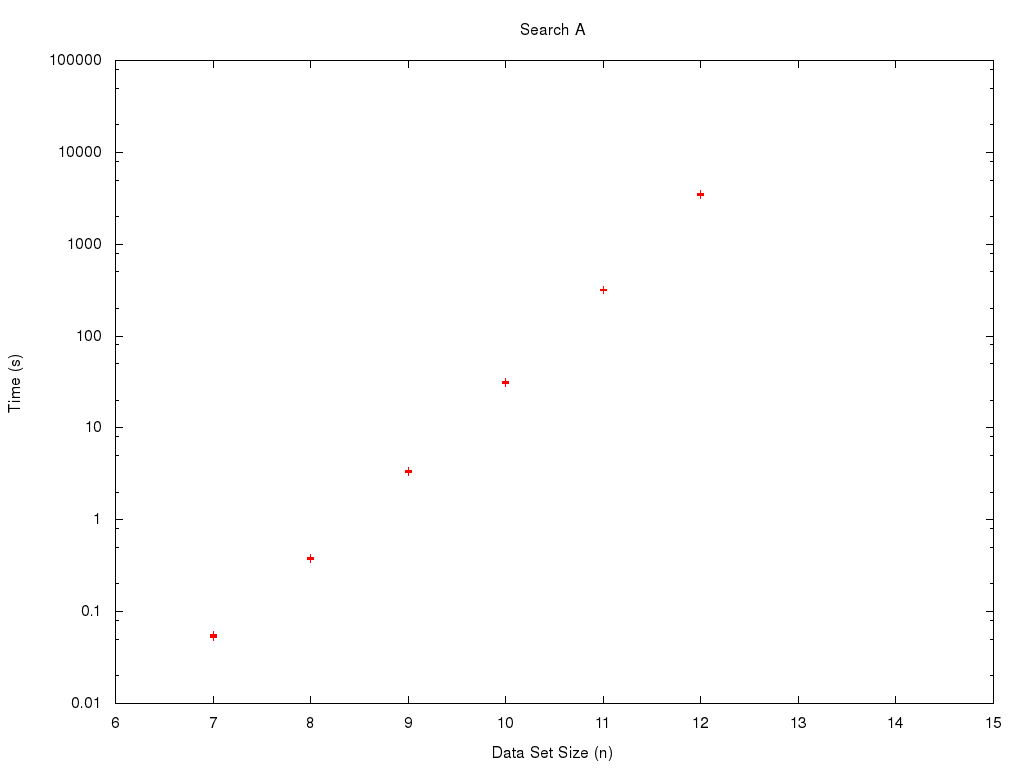
\includegraphics[width=0.8\textwidth]{../images/times_search_a.png}
	\caption{Search Time {\it vs} Problem Size, Search A}
	\label{fig:times_search_a}
\end{figure}

\begin{figure}[p]
	\centering
	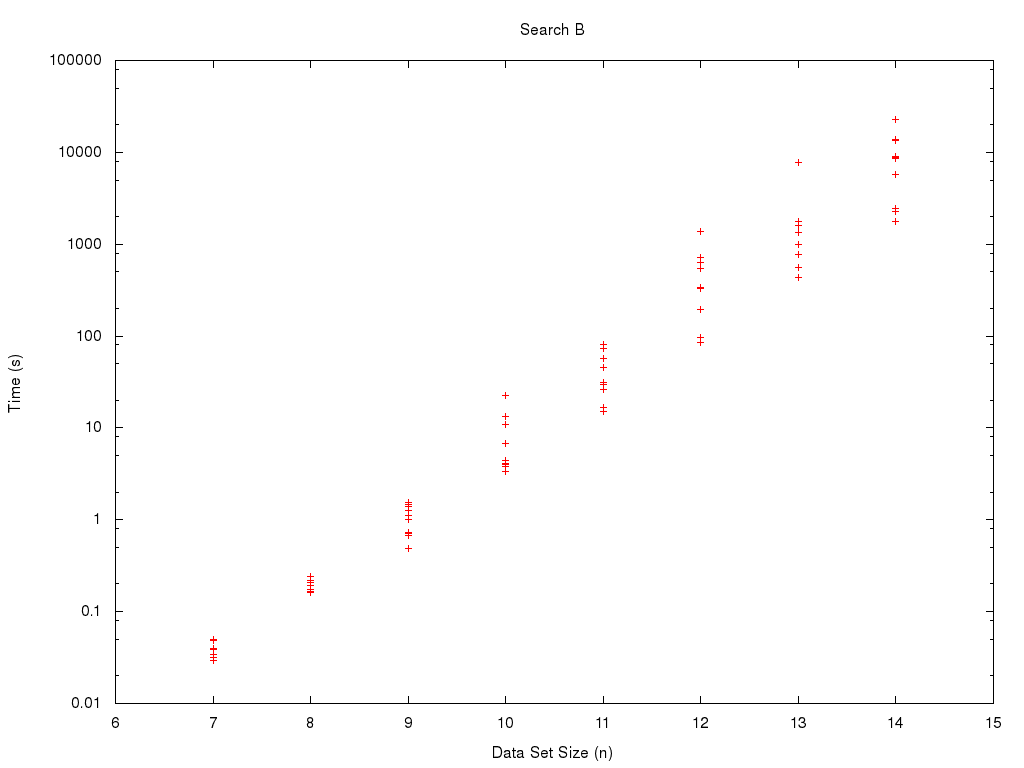
\includegraphics[width=0.8\textwidth]{../images/times_search_b.png}
	\caption{Search Time {\it vs} Problem Size, Search B}
	\label{fig:times_search_b}
\end{figure}

\begin{figure}[p]
	\centering
	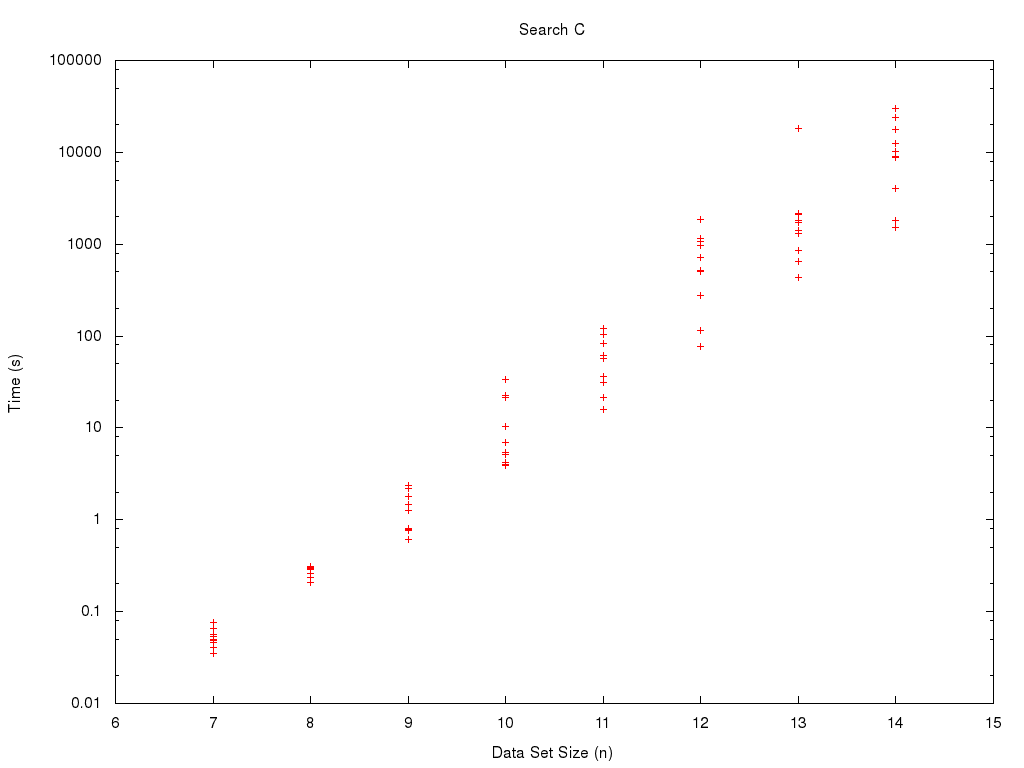
\includegraphics[width=0.8\textwidth]{../images/times_search_c.png}
	\caption{Search Time {\it vs} Problem Size, Search C}
	\label{fig:times_search_c}
\end{figure}

\begin{figure}[p]
	\centering
	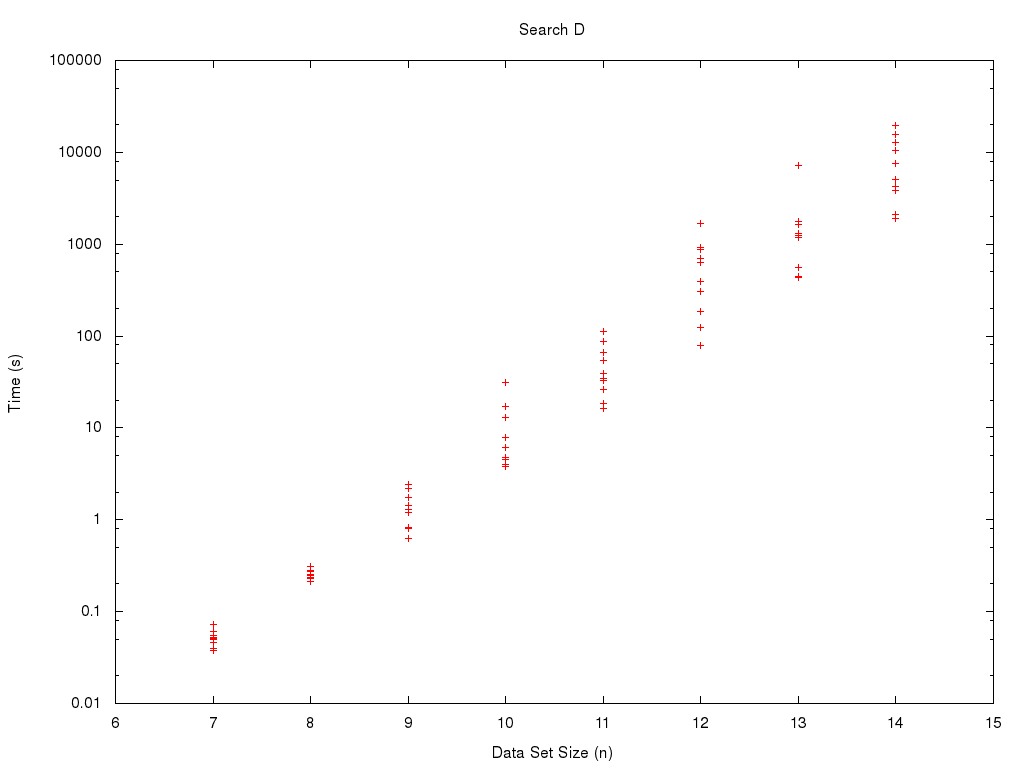
\includegraphics[width=0.8\textwidth]{../images/times_search_d.png}
	\caption{Search Time {\it vs} Problem Size, Search D}
	\label{fig:times_search_d}
\end{figure}

\begin{figure}[p]
	\centering
	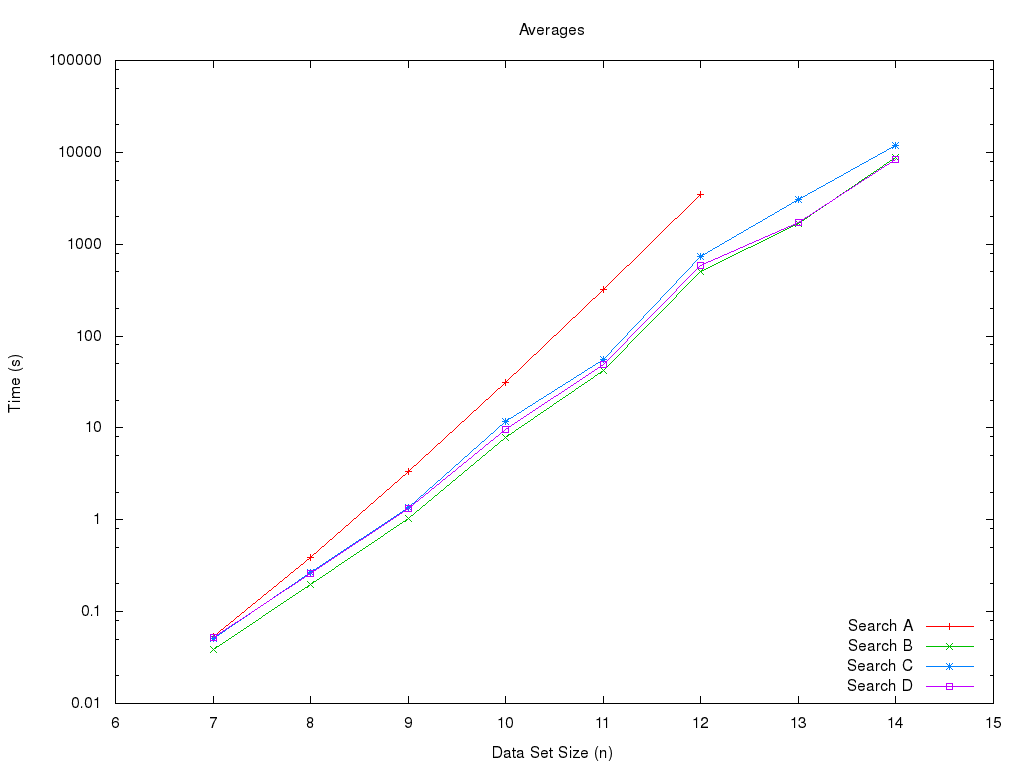
\includegraphics[width=0.8\textwidth]{../images/times_avgs.png}
	\caption{Search Time {\it vs} Problem Size, averages for all searches.}
	\label{fig:times_search_a}
\end{figure}

\begin{figure}[p]
	\centering
	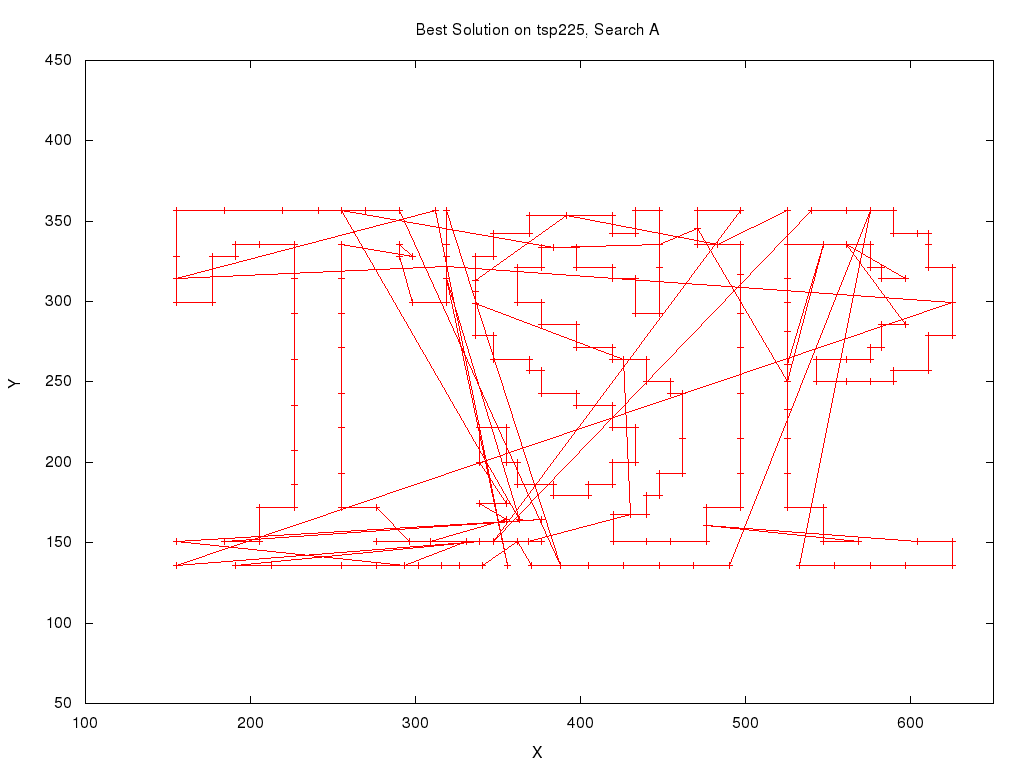
\includegraphics[width=0.8\textwidth]{../images/paths_search_a.png}
	\caption{Best Solution on {\tt tsp225.txt} found in four hours, Search A}
	\label{fig:paths_search_a}
\end{figure}

\begin{figure}[p]
	\centering
	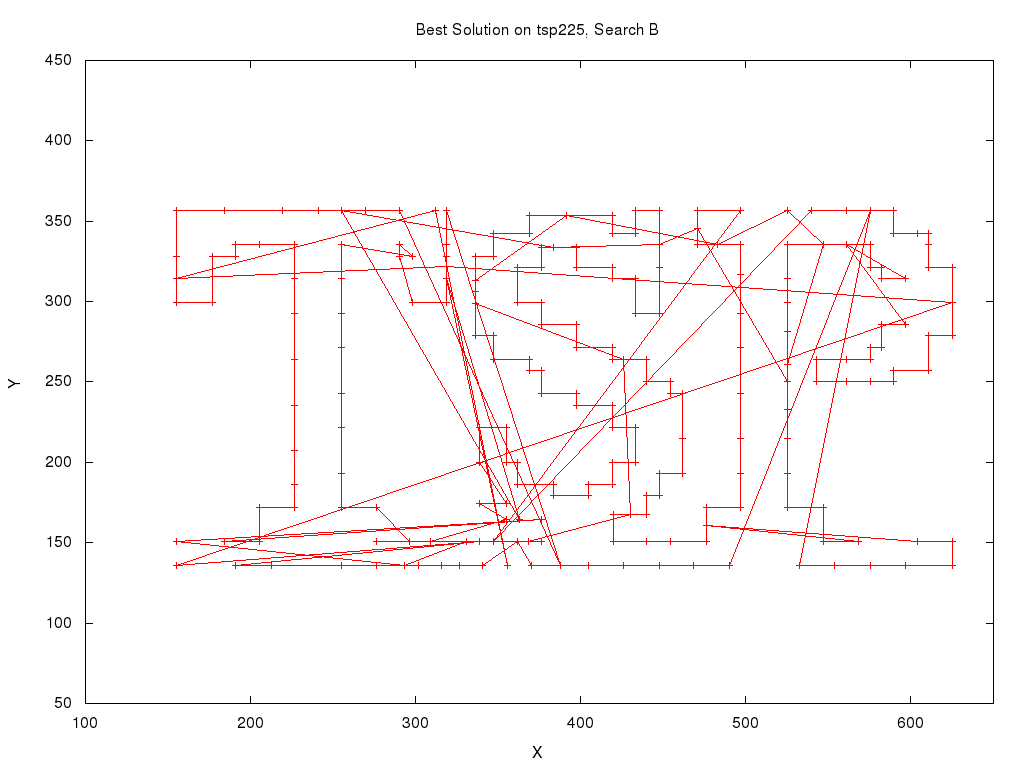
\includegraphics[width=0.8\textwidth]{../images/paths_search_b.png}
	\caption{Best Solution on {\tt tsp225.txt} found in four hours, Search B}
	\label{fig:paths_search_b}
\end{figure}

\begin{figure}[p]
	\centering
	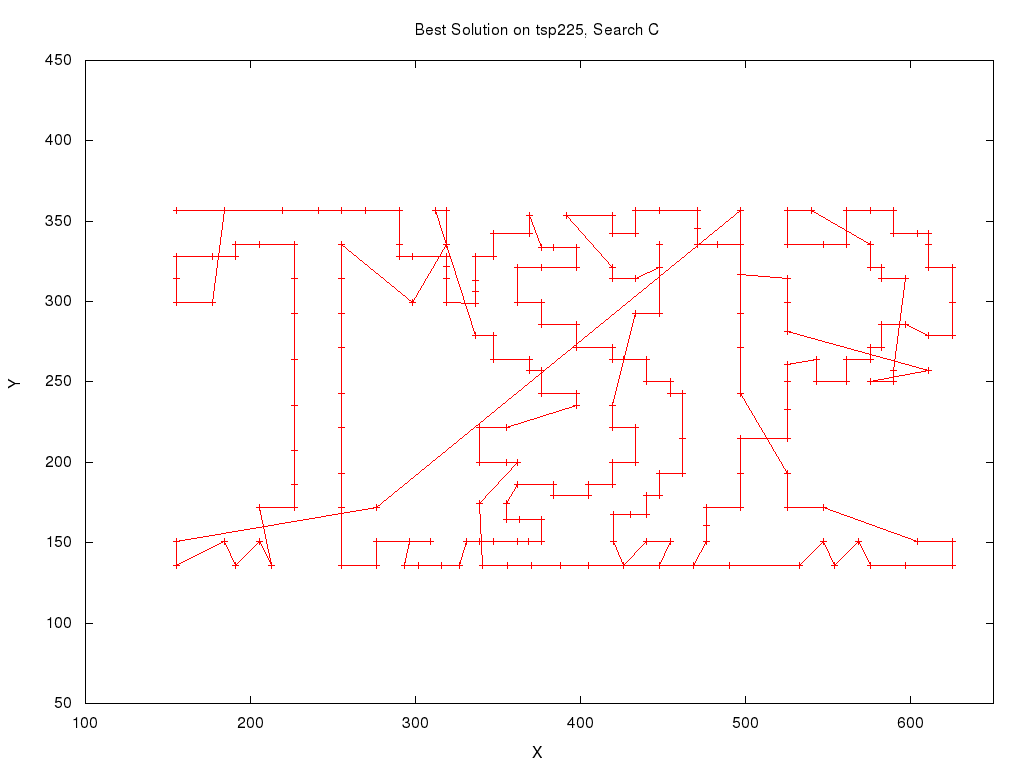
\includegraphics[width=0.8\textwidth]{../images/paths_search_c.png}
	\caption{Best Solution on {\tt tsp225.txt} found in four hours, Search C}
	\label{fig:paths_search_c}
\end{figure}

\begin{figure}[p]
	\centering
	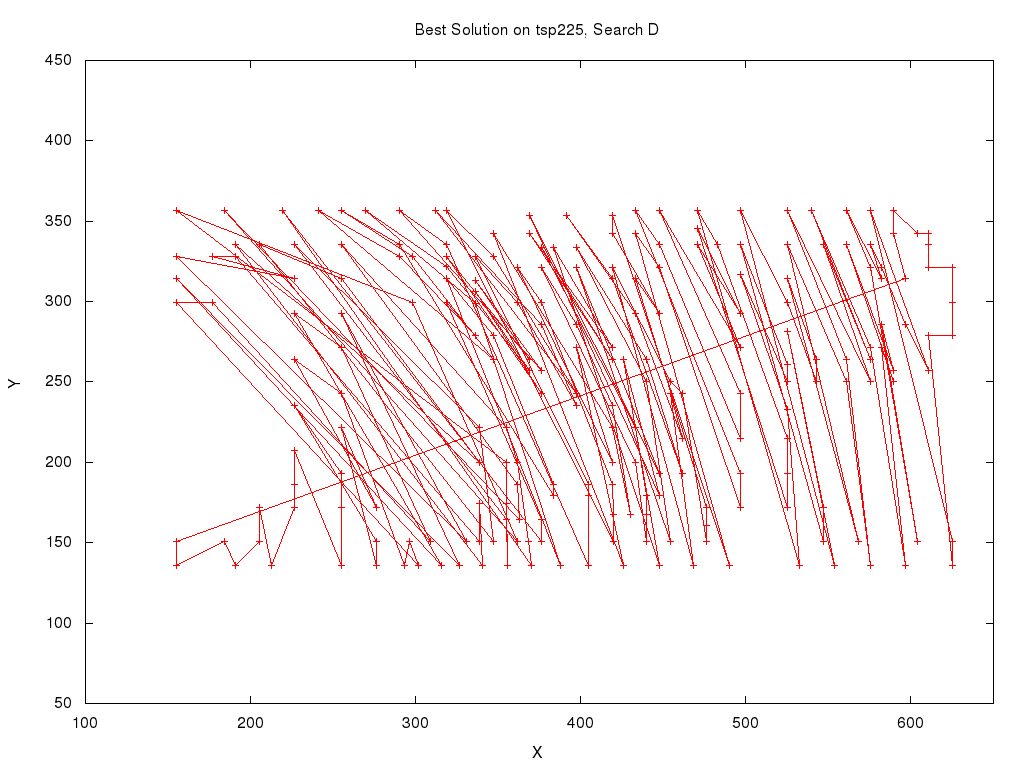
\includegraphics[width=0.8\textwidth]{../images/paths_search_d.png}
	\caption{Best Solution on {\tt tsp225.txt} found in four hours, Search D}
	\label{fig:paths_search_d}
\end{figure}

\end{document}
